% Created 2019-01-01 Tue 17:14
% Intended LaTeX compiler: pdflatex
\documentclass[letterpaper, 11pt]{article}
\usepackage[utf8]{inputenc}
\usepackage[T1]{fontenc}
\usepackage{graphicx}
\usepackage{grffile}
\usepackage{longtable}
\usepackage{wrapfig}
\usepackage{rotating}
\usepackage[normalem]{ulem}
\usepackage{amsmath}
\usepackage{textcomp}
\usepackage{amssymb}
\usepackage{capt-of}
\usepackage{hyperref}
\usepackage{minted}
\usepackage{color}
\usepackage{sidenotes}
\usepackage{minted}
\usepackage{empheq}
\usepackage{cancel}
\usepackage[top=1in, bottom=1in, right=0.5in, outer=3in, inner=0.5in, heightrounded, marginparwidth=2.5in, marginparsep=0.25in]{geometry}
\usepackage[linesnumbered,boxed]{algorithm2e}
\linespread{1.3}
\providecommand{\diff}[2]{\ensuremath{\frac{{\rm d} #1}{{\rm d} #2}}}
\providecommand{\inner}[2]{\ensuremath{\left < #1, #2 \right >}}
\providecommand{\note}[1]{\begin{margintable}{\footnotesize #1}\end{margintable}}
\providecommand{\nums}[2]{\ensuremath{\mathbb{#1}^{#2}}}
\providecommand{\abs}[1]{\ensuremath{\left | #1\right |}}
\providecommand{\On}[1]{\ensuremath{\mathcal{O}(h^{#1})}}
\providecommand{\trans}[1]{\ensuremath{{#1}^{\rm T}}}
\providecommand{\mynote}[1]{\begin{margintable}\footnotesize #1\end{margintable}}
\providecommand{\linenote}[1]{\marginnote{\footnotesize #1}}
\SetKwRepeat{Do}{do}{while}
\SetKwRepeat{Repeat}{do}{until}
\graphicspath{{./images/}}
\numberwithin{equation}{section}
\usemintedstyle{emacs}
\author{Yisu Nie}
\date{\today}
\title{Discrete Optimization -- Learning by Examples}
\hypersetup{
 pdfauthor={Yisu Nie},
 pdftitle={Discrete Optimization -- Learning by Examples},
 pdfkeywords={},
 pdfsubject={},
 pdfcreator={Emacs 25.1.1 (Org mode 9.0.3)}, 
 pdflang={English}}
\begin{document}

\maketitle
\section{Linear Algebra}
\label{sec:orgbeb4cc3}
\subsection{Matrix Decomposition}
\label{sec:org011d6e8}
\subsubsection{LU Decomposition}
\label{sec:org31bf2bf}
Lower-upper decomposition refers to the factorization of matrix \(A \in \nums{R}{m \times n}\) to a unit (diagonal elements equal to 1) lower triangular matrix
\(L\) and an upper triangular matrix \(U\): \(A = LU\).
\begin{margintable}
\textit{\footnotesize A 3 by 3 example}
\footnotesize{
\begin{align*}
&A = \left [ 
\begin{matrix}
   1 & 1 & 1 \\
4 & 3 & -1 \\
3 & 5 & 3
\end{matrix}
\right] \\
& L = \left [ 
\begin{matrix}
   1 & 0 & 0 \\
4 & 1 & 0 \\
3 & -2 & 1
\end{matrix}
\right],
U = \left [ 
\begin{matrix}
   1 & 1 & 1 \\
0 & -1 & -5 \\
0 & 0 & -10
\end{matrix}
\right]
\end{align*}
\end{margintable}
LU decomposition can be carried out using Gaussian elimination, but proper ordering of the rows (or columns) in matrix \(A\) is needed to avoid \(L\) or
\(U\) becoming singular. In practice, LU decomposition with partial pivoting allows row permutations:
\begin{equation}
\label{eq-la-lu-plu}
PA = LU,
\end{equation}
where \(P\) is \(m \times m\) permutation matrix. LU decomposition is an important vehicle for solving linear systems numerically. Starting from a generic linear system:
\begin{equation}
\label{eq-la-lu-a}
Ax=b,
\end{equation}
with Eq.\ref{eq-la-lu-plu}, we obtain
\begin{equation}
\label{eq-la-lu-b}
LUx=\widetilde{b}, \quad \widetilde{b} = Pb.
\end{equation}
Introducing an intermediate vector
\begin{equation}
\label{eq-la-lu-d}
z=Ux,
\end{equation}
then \(z\) can be solved by triangular forward-substitution:
\begin{equation}
\label{eq-la-lu-c}
Lz=\widetilde{b},
\end{equation}
and similarly \(x\) can be solved by triangular back-substitution in Eq.\ref{eq-la-lu-d}.
\paragraph{Example}
\label{sec:org07fa432}
Here we apply LU decomposition in Julia's linear algebra package with an example that \(A\) is not a square matrix. 
\begin{minted}[frame=lines,fontsize=\scriptsize,linenos]{julia}
using LinearAlgebra
A = [1 2 -3 1; 2 4 0 7; -1 3 2 0]
println("LU factorize A")
lu(A)
println("LU factorize A transpose")
lu(transpose(A))
\end{minted}

\begin{minted}[frame=lines,fontsize=\scriptsize,linenos]{julia}
3x4 Array{Int64,2}:
  1  2  -3  1
  2  4   0  7
 -1  3   2  0
LU factorize A
LU{Float64,Array{Float64,2}}
L factor:
3x3 Array{Float64,2}:
  1.0  0.0  0.0
 -0.5  1.0  0.0
  0.5  0.0  1.0
U factor:
3x4 Array{Float64,2}:
 2.0  4.0   0.0   7.0
 0.0  5.0   2.0   3.5
 0.0  0.0  -3.0  -2.5
LU factorize A transpose
LU{Float64,Array{Float64,2}}
L factor:
4x3 Array{Float64,2}:
  1.0       0.0        0.0    
 -0.333333  1.0        0.0    
 -0.666667  0.571429   1.0    
 -0.333333  0.285714  -0.13253
U factor:
3x3 Array{Float64,2}:
 -3.0  0.0  2.0     
  0.0  7.0  0.666667
  0.0  0.0  3.95238
\end{minted}

\subsubsection{Cholesky Decomposition}
\label{sec:org61f4cd8}
When matrix \(A \in \nums{R}{m \times m}\) is symmetric and positive definite, one can decompose \(A\) into the product of a lower triangular matrix \(L\)
and its transpose.
\begin{equation}
\label{eq-la-cholesky}
A = L\trans{L}.
\end{equation}
\begin{margintable}
\textit{\footnotesize symmetric matrix}
\footnotesize{
\[A = \trans{A}\]
}
\textit{\footnotesize positive definite matrix}
\footnotesize{
\[\trans{z}Az > 0, \quad \forall z \not = 0 \]
}
\end{margintable}
\subsubsection{Singular Value Decomposition}
\label{sec:org4694fd9}
Given \(m \times n\) matrix \(A\), it can be rewritten as the product of three matrices:
\begin{equation}
\label{eq-la-svd}
A = U\Sigma\trans{V},
\end{equation} 
where \(U\) is an \(m \times m\) orthogonal matrix, \(\Sigma\) is an \(m \times n\) diagonal matrix with non-negative values, and \(V\) is an \(n \times n\) orthogonal matrix.
\begin{margintable}
\textit{\footnotesize orthogonal matrix}
\footnotesize{
\trans{A}A = I}
\end{margintable}
The diagonal entries of \(\Sigma\) are the singular values, the columns of \(U\) are the left singular vectors, and the rows of \trans{V} are the right
singular vectors. The left singular vectors are eigenvectors of \(A\trans{A}\), the right singular vectors are eigenvectors of \(\trans{A}A\), and the
singular values are the square roots of the eigenvalues of \(\trans{A}A\) (or equally, \(A\trans{A}\)).
\begin{margintable}
\footnotesize{
\begin{align*}
&\trans{A}A = V\trans{\Sigma}\trans{U}U\Sigma\trans{V} = V\Sigma^2\trans{V}\\
&A\trans{A} = U\Sigma\trans{V}V\trans{\Sigma}\trans{U} = U\Sigma^2\trans{U}
\end{align*}
\end{margintable}
Geometrically, as \(A\) is a linear transformation, singular value decomposition can be interpreted as a rotation(\trans{V})-stretch(\(\Sigma\))-rotation(\(U\)) procedure.
\paragraph{Example}
\label{sec:org0b0c42b}
In this example, we use the svd function in Julia to decompose \(A \in \nums{R}{3 \times 4}\). Note that we use option \textit{full = true} to force the
program return \trans{V} as a \(4 \times 4\) matrix.
\begin{minted}[frame=lines,fontsize=\scriptsize,linenos]{julia}
using LinearAlgebra
A = [1 2 -3 1; 2 4 0 7; -1 3 2 0]
println("Singular Value Decomposition of A")
F = svd(A, full = false);
println("U")
F.U
println("V transpose")
F.Vt
println("Sigma")
Diagonal(F.S)
\end{minted}
and the result follows
\begin{minted}[frame=lines,fontsize=\scriptsize,linenos]{julia}
3x4 Array{Int64,2}:
  1  2  -3  1
  2  4   0  7
 -1  3   2  0
Singular Value Decomposition of A
U
3x3 Array{Float64,2}:
 -0.265794   0.595678   -0.757972
 -0.952144  -0.0391265   0.303135
 -0.150914  -0.80227    -0.577571
V transpose
4x4 Array{Float64,2}:
 -0.232641  -0.552221   0.0570961  -0.798542 
  0.338159  -0.351551  -0.869058    0.0824561
  0.156139  -0.746516   0.410184    0.500083 
 -0.898414  -0.119067  -0.270607    0.324728 
Sigma
3x3 Diagonal{Float64,Array{Float64,1}}:
 8.67932   ⋅        ⋅     
  ⋅       3.90259   ⋅     
  ⋅        ⋅       2.72749
\end{minted}
When use reduced size we have: 
\trans{V} = \left [
\begin{matrix}
-0.232641 & -0.552221 &  0.0570961 &  -0.798542 \\
 0.338159 & -0.351551 & -0.869058  &  0.0824561 \\
 0.156139 & -0.746516 &  0.410184  &  0.500083  \\
\end{matrix}
\right]
\section{Linear Programming}
\label{sec:org5c7b129}
\subsection{Duality}
\label{sec:orgbb24eba}
In general, duality equates two different views of the same object \cite{bertsekas2003convex}. For example, signals can be described either in the time
domain or the frequency domain. Similarly, a closed convex set \(\Omega\) can be represented by a union of internal and boundary points or by taking the
intersection of all supporting hyperplanes to \(\Omega\).
\begin{margintable}
{\footnotesize
\textit{Convex set} \\
for any $x_{1}, x_{2} \in \Omega, \theta x_{1} + (1 - \theta)x_{2} \in \Omega, \theta \in \left[0,1\right]$ \\
\textit{Supporting hyperplane} \\
for any $a \not = 0$, if hyperplane $\trans{a}x = \trans{a}x_{0}$ has the property of $\trans{a}x \leq \trans{a}x_{0}, 
\forall x \in \Omega$, then the hyperplane is a supporting hyperplane to $\Omega$ at point $x_0$ ($x_0$ is a point on the bounday of the convex set)
}
\end{margintable}
\subsubsection{Conjugate Function}
\label{sec:org7c3b7ef}
Consider a function \(f(x):\mathbb{X} \subset \nums{R}{n} \rightarrow \mathbb{R}\), its conjugate function is defined by
\begin{equation}
\label{eq-lp-dual-conjugate}
f^*(x^{*}) = \sup_{x \in \mathbb{X}} \left \{ \left< x^{*},x \right> - f(x) \right \}, \quad x^{*} \in \nums{R}{n},
\end{equation}
\begin{margintable}
{\footnotesize
\vspace{20pt}
\textit{Example of $f(x) = ax^2$}
\begin{align*}
&f^*(x^{*}) = \sup_{x} x^{*} x - ax^2 \\
&x_{argmax} = \frac{x^{*}}{2a},\quad \text{($x_{argmax}$ maximize $f(x)$})\\
&f^*(x^{*}) = \frac{x^{*}^2}{4a} 
\end{align*}
}
\end{margintable}
and the conjugate function of the conjugate can be obtained:
\begin{equation}
\label{eq-lp-dual-conjugate-2}
f^{**}(x) = \sup_{x^{*} \in \nums{R}{n}} \left\{ \left< x,x^{*} \right> - f^*(x^{*}) \right \}, \quad x \in \mathbb{X},
\end{equation}
It follows that 
\begin{equation}
\label{eq-lp-dual-conjugate-3}
f(x) \geq f^{**}(x).
\end{equation}
From Eq. \ref{eq-lp-dual-conjugate}, we have \(f(x) \geq \left< x^*,x \right> - f^*(x^*)\), which implies \(f(x) \geq \sup_{x^*} \{\left< x^*,x
\right> - f^*(x^*)\}\), where the right hand side is the definition of \(f^{**}(x)\). However, if \(f(x)\) is closed and convex, then we have \(f(x) = f^{**}(x)\).
\subsubsection{Dualization Using Perturbation}
\label{sec:orgaa40aed}
Given a general optimization problem \(\min_{x \in \mathbb{X}} f(x)\), we introduce a perturbation function \(\phi(x,y)\), where the original problem is
to minimize \(\phi(x,0)\), and the perturbed problem is to minimize \(\phi(x,y)\) for some \(y \not = 0\), also with respect to \(x\). Let
\begin{equation}
\label{eq-lp-dual-lagrangian-a}
v(y) = \inf_{x} \phi(x,y)
\end{equation}
Using the dual form \(v^{**}\) (the conjugate of the conjugate), following Eq. \ref{eq-lp-dual-conjugate-2}:
\begin{equation}
\label{eq-lp-dual-lagrangian-b}
v^{**}(y) = \sup_{y^*} \left \{ \left< y,y^* \right> - v^*(y^*) \right \}
\end{equation}
and we have equality between the primal and the dual, \(v(y) = v^{**}(y)\). When we set \(y = 0\), the dual form of the optimization
problem reduces to
\begin{equation}
\label{eq-lp-dual-lagrangian-b}
v^{**}(0) = \sup_{y^*} \left \{- v^*(y^*) \right \}
\end{equation}
Now we consider the convex conjugate of the pertured function \(\phi(x,y)\):
\begin{equation}
\label{eq-lp-dual-phi-conjugate}
\phi^{*}(x^*,y^*) = \sup_{x, y} \left \{ \left< x^*,x \right> + \left< y^*,y \right> - \phi(x,y) \right \}
\end{equation}
When we choose \(x^* = 0\), we obtain
\begin{subequations}
\label{eq-lp-dual-phi-conjugate-v}
\begin{align}
\phi^{*}(0,y^*) & = \sup_{x, y} \left \{ \inner{y^*}{y} - \phi(x,y) \right \} \\
& = \sup_{y} \left \{ \inner{y^*}{y} - \inf_{x}\phi(x,y) \right \} \\
& = \sup_{y} \left \{ \inner{y^*}{y} - v(y) \right \} \\
& = v^*(y^*)
\end{align}
\end{subequation}
Now, we can have the dual problem stated as
\begin{equation}
\label{eq-lp-dual-primal-dual}
\mathbf{\phi(x,y = 0)} = v(0) = v^{**}(0) = \sup_{y^*} \left \{- v^*(y^*) \right \} = \mathbf{\sup_{y^*} \left \{ -\phi^*(x^*=0,y^*) \right \}}
\end{equation}
\begin{margintable}
{\footnotesize
Assuming strong duality here $v(0) = v^{**}(0)$. Otherwise, for weak duality $v(0) > v^{**}(0)$. Also, keeping the minus sign in the end for later convenience in deriving Lagrangian.
}
\end{margintable}
\paragraph{Lagrangian Dual}
\label{sec:org9024d9b}
Consider the general form of a convex optimization problem as follows:
\begin{subequations}
\label{eq-lp-dual-lagrangian}
\begin{align}
&\min \, f(x)  \\
&s.t. \quad h(x) = 0 \\
&\qquad \,\, g(x) \leq 0
\end{align}  
\end{subequations}
and a perturbed problem\mynote{Every dualization in optimization is associated with a perturbation function}
\begin{subequations}
\label{eq-lp-dual-lagrangian-perturbed}
\begin{align}
&\min \, f(x)  \\
&s.t. \quad h(x) + y_{1} = 0 \\
&\qquad \,\, g(x) + y_{2} \leq 0
\end{align}  
\end{subequations}
With the pertubation specified in Eq. \ref{eq-lp-dual-lagrangian-perturbed}, we define function \(\phi\) as
\begin{equation}
\label{eq-lp-dual-phi-lagrangian}
\phi(x,y_1,y_2) = 
\left\{
\begin{array}{ll}
      f(x) & h(x) + y_{1} = 0, g(x) + y_{2} \leq 0 \\ 
      \infty & \text{otherwise}\\
\end{array} 
\right. 
\end{equation}
By definition in Eq. \ref{eq-lp-dual-phi-conjugate}, one writes
\begin{subequations}
\label{eq-lp-dual-lagrangian-dual}
\begin{align}
-\phi^{*}(x^*=0,y_1^*,y_2^*) & = -\sup_{ \tiny
\begin{aligned}
&x \in \mathbb{X}\\
&h(x) + y_1 = 0\\
&g(x) + y_2 \leq 0 
\end{aligned}
} \left \{ \inner{0}{x} + \inner{y_1^*}{y_1} + \inner{y_2^*}{y_2} - f(x) \right \} \\
& = -\sup_{x,z\geq 0} \left \{ \inner{y_1^*}{-h(x)} + \inner{y_2^*}{-g(x)-z} - f(x)  \right \} \\
& = 
\left\{
\begin{array}{ll}
      \inf_{x} \left\{ f(x) + \inner{y_1^*}{h(x)} + \inner{y_2^*}{g(x)} \right \} & $y_2^*\geq 0$\\
      \infty & \text{otherwise}\\
\end{array} 
\right. 
\end{align}
\end{subequation}
\begin{margintable}
{\footnotesize
Sign of $y^*_2$ has to be non-negative. Otherwise, $\inner{y_2^*}{z}$ becomes unbounded below.  
}
\end{margintable}
To this end, we recogozie the \textbf{Lagrangian function} (with slight variation in notation from above):
\begin{equation}
\label{eq-lp-dual-lagrangian-function-final}
\mathcal{L}(x,\mu, \lambda) = f(x) + \trans{\mu}{h(x)} + \trans{\lambda}{g(x)},
\end{equation}
and the \textbf{Lagrangian dual function} is 
\begin{equation}
\label{eq-lp-dual-lagrangian-dual-function-final}
g(\mu, \lambda) = \inf_{x} \left \{ f(x) + \trans{\mu}{h(x)} + \trans{\lambda}{g(x)} \right \},
\end{equation}
and the \textbf{Lagrangian dual problem} is
\begin{equation}
\label{eq-lp-dual-lagrangian-dual-problem-final}
\sup_{\mu, \lambda} g(\mu, \lambda).
\end{equation}
\subsubsection{Linear Programming Duality}
\label{sec:org87a3df9}
Now we apply Lagrangian duality to derive the dual of linear program:
\begin{subequations}
\label{eq-lp-dual-primal}
\begin{align}
&\max \, \trans{c}x  \\
&s.t. \quad Ax \leq b \\
&\qquad \,\, x \geq 0
\end{align}  
\end{subequations}
\begin{margintable}
{\footnotesize
Define the Lagrangian:
\begin{align*}
&\mathcal{L}(x,\lambda,\mu) = -\trans{c}x + \trans{\lambda}\left ( Ax - b\right) - \trans{\mu}x\\
&\lambda \geq 0,\quad \mu \geq 0
\end{align*}
Stationary condition w.r.t. $x$, requires 
\[
-\trans{c} + \trans{\lambda}A - \trans{\mu} = 0
\]
and the Lagrangian dual function becomes
\[
g(\lambda, \mu) = \left ( -\trans{c} + \trans{\lambda}A - \trans{\mu} \right)x -\trans{\lambda}b = -\trans{\lambda}b 
\]
}
\end{margintable}
and the dual problem using the Lagrangian is 
\begin{subequations}
\label{eq-lp-dual-dual-intermediate}
\begin{align}
&\max \, -\trans{\lambda}b  \\
&s.t. \quad -\trans{c} + \trans{\lambda}A - \trans{\mu} = 0  \\
&\qquad \,\, \lambda \geq 0,\quad \mu \geq 0
\end{align}  
\end{subequations} 
Rearranging terms and substitute out \(\mu\), we end up with the classic form of the dual to the liner program \ref{eq-lp-dual-primal}:
\begin{subequations}
\label{eq-lp-dual-dual-intermediate}
\begin{align}
&\min \, \trans{b}\lambda  \\
&s.t. \quad \tans{A}\lambda \geq c \\
&\qquad \,\, \lambda \geq 0
\end{align}  
\end{subequations} 
\section{Lagrangian Relaxation\hfill{}\textsc{Completed}}
\label{sec:orga6a4cda}
\subsection{Theory}
\label{sec:org5df3f82}
\subsubsection{Basic Theorem}
\label{sec:org0a57057}
Lagrangian relaxation \mynote{Aslo spell as Lagrangean relaxation} is a constraint decomposition method, where model constraints are separated to an
easy and a hard group. The reduced problem with the subset of the easy constraints can be solved rapidly in practice. Consider an integer program as
follows:
\begin{subequations}
\label{eq-lr-ip-formulation}
\begin{align}
&z_{IP} = \min \, cx  \\
\label{eq-lr-bad-cons}
&s.t. \quad Ax \geq b \\
\label{eq-lr-nice-cons}
&\qquad \,\, Dx \geq e \\
&\qquad \,\, x \in \mathbb{Z}^{n}_{+} 
\end{align}  
\end{subequations}
The complicating (bad) constraints in Eq. \eqref{eq-lr-bad-cons} can be cast to the objective function with a pricing variable \(u\) to try to ensure
feasibility.
\begin{subequations}
\begin{align}
&z_{LR} = \min \, cx + u(b - Ax) \\
&s.t. \quad Dx \geq e \\
&\qquad \,\, x \in \mathbb{Z}^{n}_{+} 
\end{align}  
\end{subequations}
\(z_{LR}\) is called the Lagrangian relaxation of the original integer program \(z_{IP}\), and \(z_{LR}\) is an underestimate of \(z_{IP}\). For a quick
proof, assuming \(x^{*}\) is the optimal solution of the integer program:
\begin{subequations}
\begin{empheq}{align}
& z_{IP} = cx^{*} \geq cx^{*} + u(b-Ax^{*}) \marginnote{\footnotesize $x^*$ is feasible in IP $\rightarrow b-Ax^*\leq 0$ and $u \geq 0$}\\ 
& cx^{*} + u(b-Ax^{*}) \geq cx + u(b- Ax) = z_{LR} \marginnote{\footnotesize $x^*$ is feasible in LR}\\
& z_{IP} \geq z_{LR} 
\end{empheq}
To obtain the best lower bound, we search the space of the dual vector $u$, and introduce the Lagrangian dual:
\begin{subequations}
\begin{align}
&z_{LD} = \max_{u \geq 0} z_{LR} = \max_{u \geq 0} \min_{x} cx + u(b-Ax) \\
&s.t. \quad Dx \geq e \\
&\qquad \,\, x \in \mathbb{Z}^{n}_{+} 
\end{align}
\end{subequations}
\subsubsection{Advanced Theorem}
\label{sec:org1edfe4d}
The remaining constraint set after the transformation can be denoted as \(Z = \{\mathbb{Z}^{n}_{+}:\, Dx \geq e\}\). If this set contains a finite
number of (extreme or integer) points \(t =1,\ldots,T\). The Lagrangian dual can be viewed alternatively as:
\begin{equation}
\label{eq-ldual-ip-formulation}
z_{LD} = \max_{u \geq 0} z_{LR} = \max_{u \geq 0} \min_{t=1,\ldots,T} cx^{t} + u(b-Ax^{t}).
\end{equation}
This can be rewritten to a linear program: 
\begin{subequations}
\begin{empheq}{align}
&z_{LD} = \max \mu \\
&s.t. \quad \mu - u(b-Ax^t) \geq cx^t, \quad t=1,\ldots,T, \marginnote{\footnotesize $\mu$ is the smallest value among t}\\
&\qquad \,\, u \geq 0, \mu \in \mathbb{R}^{1}
\end{empheq}
\end{subequations}
Introducing \(\lambda^{t}\) as the dual variables for the constraints, the dual of the linear program can be deduced: 
\begin{subequations}
\begin{empheq}{align}
&z_{LD} = \min \sum_{t=1}^{T} (cx^t)\lambda^{t} \\
&s.t. \quad \sum_{t=1}^{T} \lambda^{t} = 1 \\
&\qquad \,\, \sum_{t=1}^{T} (Ax^t) \lambda^{t} \geq b,\marginnote{\footnotesize $\sum_{t=1}^{T}\lambda^{t}b = b$} \\
&\qquad \,\, \lambda \in \mathbb{R}^{T}_{+}
\end{empheq}
\end{subequations}
With this form, the Lagrangian dual can be further expressed as 
\begin{equation}
\label{eq-ldual-lp-formulation}
z_{LD} = \min\{cx:\, Ax \geq b, x \in conv(Z)\}
\end{equation}
The convex hull of set \(Z\) is defined by the extreme points \(x^{t}\), noted as
\begin{equation}
conv(Z) = \{x:\, x = \sum_{t=1}^{T} x^t\lambda^t, \sum_{t=1}^{T} \lambda^t = 1, \lambda^t \geq 0\}
\end{equation}
Comparing the above formulation in Eq. \ref{eq-ldual-lp-formulation} with the IP problem in Eq. \ref{eq-lr-ip-formulation}, one can view the Lagrangian
dual problem as optimizing the objective function within the intersection of the complicating constraints and the convex hull of the easy constraints.
\subsection{Algorithm}
\label{sec:org0d09789}
\subsubsection{Subgradient Algorithm}
\label{sec:org07773a6}
\begin{margintable}
\footnotesize
\textit{Subgradient at $x=0$}\\
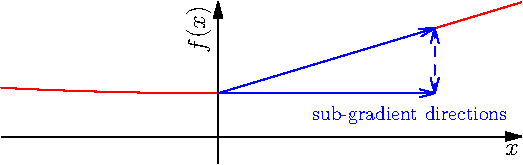
\includegraphics[scale=0.7]{lagrangian-relaxation-sub-gradient}
For any function $f(x)$ (no need to be convex), if 
\[
f(x) - f(x_0) \geq s^{T}(x - x^0), \quad \forall x
\]
Then $s^T$ is a subgradient at $x=x_0$.
\vspace{10pt}
\end{margintable}
The Lagrangian dual (LD) function in Eq. \eqref{eq-ldual-ip-formulation} is a maximization problem over a piece-wise affine and concave function. However,
the function is non-differentiable \cite{junger200950}. The subgradient algorithm can be used to solve this problem. The algorithm is stated in
Algorithm \ref{ag-lr-sub-gradient}:
\begin{margintable}
\footnotesize
The subgradient algorithm was first developed by Shor \cite{shor1962application}. The convergence property is governed by the step size law. 
A formula that has been proved effective was proposed in \cite{held1974validation}:
\[
\begin{aligned}
&\gamma^{t} = \alpha^{t}\frac{z^*_{IP}-z_{LR}(u^t)}{\lVert b-Ax^{t} \rVert};\\
&\alpha^{t} = 
\begin{cases}
    2,  & $t=0$; \\
    0.5\alpha^{t-1}, & \text{$z_{LR}(u^t)$ $N^{\rm th}$ decrease failure} \\
    \alpha^{t-1}, &\text{else}.
\end{cases}
\end{aligned}
\]   
Here, $\lVert b-Ax^{t} \rVert := \sum_{i}(b_{i} - \sum_{j}a_{ij}x^{t})^2$. And $z^*_{IP}$ can be replaced by any known values (obtained from feasible solutions).
This update formula does not guarantee convergence to optimality \cite{fisher1985applications}. 
\end{margintable}
\begin{algorithm}
\caption{Subgradient algorithm for solving the Lagrangian dual}
\label{ag-lr-sub-gradient}
Initial guesses of dual solution $u^{0}=0$ and primal solution $x^{0}$ \;
Set iteration index $t=1$\;
\Do{Change in the multiplier $\abs{u^{t} - u^{t-1}} > \tau$ ($\tau$ is a small positive number) and $t < t^{max}$ ($t^{max}$ represents maximum iteration number)}
{
 Solve Lagrangian relaxation problem in Eq. \eqref{eq-lr-ip-formulation} to obtain the lower/dual bound and optimal solution $x^{t}$ \;
 Compute subgradient $s^{t} = b - Ax^{t}$\;
 Update dual solution $u^{t+1} = \max \{0, u^{t} + \gamma^{t}s^{t}\}$. 
 This update means moving along the subgradient direction with a step size controlled by coefficient $\gamma^{t}$\; 
}
Best solution at algorithm termination $u^{t^*}$, $x^{t^*}$.
\end{algorithm}
\subsection{Example}
\label{sec:org479bf44}
The illustrative example we use is modified from the example given by Fisher \cite{fisher1985applications}. The implementation of the example IP in
Julia/JuMP is shown as below
\begin{minted}[frame=lines,fontsize=\scriptsize,linenos]{julia}
using JuMP
@time begin
c = [-16, -10, 0, -4]
A = [-8, -2, -1, -4]
B1 = [-1, -1, 0, 0]
B2 = [0, 0, -1, -1]

ip = Model() 
@variable(ip, x[1:4], Bin)
@objective(ip, Min, dot(c,x))
@constraint(ip, dot(A,x) >= -10)
@constraint(ip, dot(B1,x) >= -1)
@constraint(ip, dot(B2,x) >= -1)
opt = solve(ip)
end
print(ip)
println("Model status: ", opt, " | Objective value: ", getobjectivevalue(ip))
println("x = ", getvalue(x))
\end{minted}
The IP can be solved to optimality using open-source solver CBC \cite{forrest2005cbc} from COIN-OR, with the best objective function value at \(-16\).
\begin{margintable}
\footnotesize
Computational Infrastructure for Operations Research (https://www.coin-or.org/)
 website hosts a collection of open-source software for scientific computing, in particular mathematical optimization. 
\end{margintable}
\begin{minted}[frame=lines,fontsize=\scriptsize,linenos]{julia}
  1.910062 seconds (611.85 k allocations: 26.214 MB, 0.38% gc time)
Min -16 x[1] - 10 x[2] - 4 x[4]
Subject to
 -8 x[1] - 2 x[2] - x[3] - 4 x[4] >= -10
 -x[1] - x[2] >= -1
 -x[3] - x[4] >= -1
 x[i] in {0,1} for all i in {1,2,3,4}
Model status: Optimal | Objective value: -16.0
x = [1.0,0.0,0.0,0.0]
\end{minted}
The Lagrangian subproblem is created by relaxing the first constraint---it is the complicating constraint since all the decision variables
appear---and shift the relaxed constraint to the objective function with the penalty factor \(u\). We set the initial guess of \(u=0\), which in fact is
equivalent to dropping the constraint.
\begin{minted}[frame=lines,fontsize=\scriptsize,linenos]{julia}
using JuMP
c = [-16, -10, 0, -4]
A = [-8, -2, -1, -4]
B1 = [-1, -1, 0, 0]
B2 = [0, 0, -1, -1]
u = 0

lr = Model() 
@variable(lr, x[1:4], Bin)
@objective(lr, Min, dot(c,x) + u*(-10 - dot(A,x)))
@constraint(lr, dot(B1,x) >= -1)
@constraint(lr, dot(B2,x) >= -1)
opt = solve(lr)
print(lr)
println("u = ", u)
println("Model status: ", opt, " | Objective value: ", getobjectivevalue(lr))
println("x = ", getvalue(x))
\end{minted}
The solution we obtain with the relaxed problem is lower than the true optimum as expected, and the optimal value of the decision variable is
different.
\begin{minted}[frame=lines,fontsize=\scriptsize,linenos]{julia}
Min -16 x[1] - 10 x[2] - 4 x[4]
Subject to
 -x[1] - x[2] >= -1
 -x[3] - x[4] >= -1
 x[i] in {0,1} for all i in {1,2,3,4}
u = 0
Model status: Optimal | Objective value: -20.0
x = [1.0,0.0,0.0,1.0]
\end{minted}
To search for the true optimal solution with the subgradient algorithm, we introduce the relaxed subproblem:
\begin{minted}[frame=lines,fontsize=\scriptsize,linenos]{julia}
  using JuMP
  using Gadfly
  using DataFrames

  # model parameters
  c = [-16, -10, 0, -4]
  A = [-8, -2, -1, -4]
  B1 = [-1, -1, 0, 0]
  B2 = [0, 0, -1, -1]

  function solve_lagrangian_sub(u)
      lr = Model() 
      x = @variable(lr, [1:4], Bin)
      @objective(lr, Min, dot(c,x) + u*(-10 - dot(A,x)))
      @constraint(lr, dot(B1,x) >= -1)
      @constraint(lr, dot(B2,x) >= -1)
      opt = solve(lr)
      return opt, getobjectivevalue(lr), getvalue(x) 
  end

  function calc_step(t, u_old, s, PB, lr_obj, lr_obj_old, alpha_old, no_impr)
      # check objective value improvement
      if lr_obj < lr_obj_old
          no_impr = no_impr + 1
      else
          no_impr = 0
      end
      # calculate step size alpha
      if no_impr > 0
          alpha = 0.5*alpha_old
      else
          alpha = alpha_old
      end
      # calculate gradient 
      g = (PB - lr_obj)/s^2
      u = max(0, u_old + s*alpha*g)
      t = t + 1
      return u, t, alpha, no_impr
  end

  t = 0
  LB = []
  UB = []
  while t <= 200
      # first iteraion
      if t == 0
          u = 0
          _, obj, x = solve_lagrangian_sub(u)
          alpha = 2
          obj_old = obj
          no_impr = 0 
          PB = 0
          best = Inf
      end
      append!(LB, obj)
      # calculate subgradient and check convergence
      s = -10 - dot(A, x)
      if abs(s) < 1e-3
          break
      end
      # update best feasible solution
      if s <= 0
          best = min(best, obj-u*s)
      end
      append!(UB, best)
      # update u 
      u, t, alpha, no_impr = calc_step(t, u, s, PB, obj, obj_old, alpha, no_impr)
      # record previous objective function value
      obj_old = obj
      # solve Lagrangian subproblem
      opt, obj, x = solve_lagrangian_sub(u)
  end

df1 = DataFrame(x=2:length(UB), y=convert(Array{Float64,1}, UB[2:end]), bound="Upper")
df2 = DataFrame(x=2:length(LB), y=convert(Array{Float64,1}, LB[2:end]), bound="Lower")
df = vcat(df1, df2);

  my_plot = plot(df, x=:x, y=:y, color=:bound, Geom.step, Guide.xlabel("Iteration"), Guide.ylabel("Objective"));
  draw(PDF("./images/lagrangian-relaxation-sub-gradient-converge.pdf", 3inch, 3inch), my_plot)
\end{minted}

\begin{figure}[htbp]
\centering
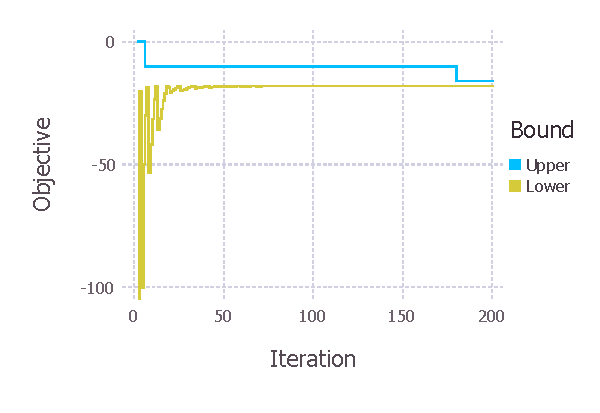
\includegraphics[width=.85\linewidth]{images/lagrangian-relaxation-sub-gradient-converge.pdf}
\caption{\label{fig:org14b2f4b}
Convergence plot of the subgradient algorithm}
\end{figure} 
After 200 iterations, the best lower bound obtained is \(-18\), and the best upper bound is
\(-16\) (which is the optimal solution).  It is worth noting that the Lagrangian relaxation is as good as the linear programming relaxation of the
original IP. LP relaxation is obtained by solving the same IP problem with relaxed integrality constraints, where in Julia/JuMP we can use \mintinline{julia}\{solve(model,
relaxation=true)\}.
\section{Benders' Decomposition\hfill{}\textsc{Wait}}
\label{sec:org73faf76}
\subsection{Theory}
\label{sec:org3c24aa1}
\subsubsection{Basic Theorem}
\label{sec:orge2a3957}
Benders' Decomposition is a variable-based decomposition scheme, firstly proposed to address mixed-integer programs (MIPs)
\cite{benders1962partitioning}. Consider a typical MIP in the follwing form: 
\begin{subequations}
\label{eq-bd-mip-formulation}
\begin{align}
&z_{MIP} = \min \, cx + dy \\
&s.t. \quad Ax + By \geq e \\
&\qquad \,\, x \in \mathbb{Z}_{+}^{m}, y \in \mathbb{R}_{+}^{n} 
\end{align}  
\end{subequations}
Benders' Decomposition algorithm for MIPs is based on projection methods, where the feasible region of the MIP \(Q_{0} = \left\{(x,y) \in
\mathbb{Z}_{+}^{m} \times \mathbb{R}_{+}^{n} \right\}\) is reformulated to a lower dimensional domain with only the discrete variables and a single
continuous variable \(Q_{r} = \{(x,\sigma) \in \mathbb{Z}^{m} \times \mathbb{R}\}\).
\begin{margintable}
\textit{\footnotesize Project of polyhedron $P$}
\footnotesize{
\begin{align*}
&\text{For }P = \left \{ (x,y) \in \mathbb{R}^{m} \times \mathbb{R}^{n} \right \}, \\
&\text{Projection onto the x space } \\
&Proj_{x}(P) = \left \{ x \in \mathbb{R}^{m}: \exists y \in \mathbb{R}^{n} \text{that} (x,y) \in P \right \}
\end{align*}
}
\end{margintable}
To derive such a projection, consider solving the the subproblem as a linear problem with integer variables fixed at \(x = {\bar x}\):
\begin{subequations}
\label{eq-bd-slp-formulation}
\begin{empheq}{align}
&z_{SLP} = \min dy\, \cancel{+\, c{\bar x}} \linenote{Dropped constant term with fixed integers} \\
&s.t. \quad By \geq e - A{\bar x} \\
&\qquad \,\, y \in \mathbb{R}_{+}^{n} 
\end{empheq}
\end{subequations}
Now consider the dual problem of \(z_{SLP}\):
\begin{subequations}
\label{eq-bd-dslp-formulation}
\begin{empheq}{align}
&z_{DSLP} = \max u(e - A{\bar x}) \\
&s.t. \quad uB \leq d \linenote{Feasible region does NOT depend on $x$ value}\\
&\qquad \,\, u \in \mathbb{R}_{+}^{p} 
\end{empheq}
\end{subequations}
From LP duality, if \(z_{SLP}\) is feasible, it follows that 
\begin{equation}
\label{eq-bd-lp-duality-feasible}
\sigma = z_{SLP} = z_{DSLP} = \max_{t = 1,\ldots,T} u^t(e - A{\bar x}),
\end{equation} 
where \(u^t\) are the extreme points of \(U = \{u \in \mathbb{R}_{+}^{p}:uB \leq d\}\). On the other hand, infeasible \(z_{SLP}\) suggests that \(\exists v
\in V\) such that \(v(e - A{\bar x}) > 0\).
\begin{margintable}
\footnotesize
This is a result from Farkas Lemma and $V = \{ v \in \mathbb{R}_{+}^{p}:uB \leq 0 \}$
\end{margintable}
The infeasible instances can be suppressed by augmenting constriants \(v(e - A{\bar x}) \leq 0, \forall v \in V\), which are equivalent to 
\linenote{Extreme rays of $V$ and $U$ are the same if they are not empty.} 
\begin{equation}
v^{r}(e -A{\bar x}) \leq 0, \quad r = 1,\ldots, R,
\end{equation}
when \(v^{r}\) are the extreme rays of \(V\). To this end, the reformulated MIP problem can be stated as
\begin{subequations}
\label{eq-bd-rmip-formulation}
\begin{empheq}{align}
&z_{RMIP} = \min \, cx + \sigma \\
&s.t. \quad  u^t\left (e - Ax\right ) \leq \sigma, \quad t = 1,\ldots, T \linenote{$\sigma$ is the maximum as shown in Eq.~\eqref{eq-bd-lp-duality-feasible}}\\ 
&\qquad \,\, v^r\left (e - Ax\right ) \leq 0, \quad r = 1,\ldots, R \\
&\qquad \,\, x \in \mathbb{Z}_{+}^{m} \linenote{Constraints apply to all $x \in \mathbb{Z}_{+}^{m}$}
\end{empheq}  
\end{subequations}
If the orginal problem \(z_{MIP}\) is feasible and bounded, \(z_{MIP}\) and \(z_{RMIP}\) are equivalent. However, the number of constraints in the
reformulated problem Eq. \ref{eq-bd-rmip-formulation} are very large in genernal.
\begin{margintable}
\footnotesize
Exhaustive enumeration over extreme points and rays of $U = \{u \in \mathbb{R}_{+}^{p}:uB \leq d\}$ is very expensive, if not prohitive$}.
\end{margintable}
A typical strategy is to relax the feasible region by considering a subset of extreme points and rays, and gradually add constraints to
improve the relaxation in an iterative procedure. The relaxed version of \(z_{RMIP}\) is employed the master problem in the Benders' Decomposition
scheme, denoted as 
\begin{subequations}
\label{eq-bd-master-formulation}
\begin{empheq}{align}
&z_{MP} = \min \, cx + \sigma \\
&s.t. \quad  u^t\left (e - Ax\right ) \leq \sigma, \quad t = 1,\ldots, T_r \linenote{$T_r \leq T$} \\\ 
&\qquad \,\, v^r\left (e - Ax\right ) \leq 0, \quad r = 1,\ldots, R_r \linenote{$R_r \leq R$}\\
&\qquad \,\, x \in \mathbb{Z}_{+}^{m} 
\end{empheq}  
\end{subequations}    
\subsubsection{Extended Forms}
\label{sec:org2f1fc45}
\paragraph{Logic Based Benders' Decomposition}
\label{sec:orgbe01cbd}
\paragraph{Generalized Benders' Decomposition}
\label{sec:org0e4960a}
\subsection{Algorithm}
\label{sec:orgff7c735}
Benders' Decomposition is a flexible solution paradigm that can be implemented in a various forms. In the following discussion, we assume the use of
the dual form in subproblems.
\subsubsection{Classic Implementation}
\label{sec:orgb1aaa01}
The classic implementation presented in the following, iterates over the master problem \(z_{MP}\) and the subproblem \(z_{DSLP}\).
\begin{algorithm}
\caption{Classic Benders' Decomposition algorithm}
\label{ag-bd-classic}
Set iterator $i=1$ and initial guess of integer assignment $x^{1}$\;
Set the upper bound $UB = \infty$ and the lower bound $LB = -\infty$\;
\While{Gap between bounds $\abs{UB - LB} > \tau$ ($\tau$ is a small positive number)}
{
 Solve the subproblem in Eq. \eqref{eq-bd-dslp-formulation} at $x^{i}$ to obtain the lower/dual bound and optimal solution $x^{t}$ \;
 \uIf{optimal solution at $u^{i}$}{Add an optimality cut $u^i\left (e - Ax\right ) \leq \sigma$ to $z_{MP}$\; Update $UB = \min \{UB, u^i(e - Ax^i)\}$}
 \uElseIf{unbounded solution}{Add a feasibility cut $v^i\left (e - Ax\right ) \leq 0$ to $z_{MP}$ \;}
 Solve the master problem in Eq. \eqref{eq-bd-master-formulation} with generated cuts, with the optimal solution $x^*$ and $\sigma^*$ \;
 Update $LB = cx^* + \sigma^*$ \;
 Set $i = i + 1$, $x^{i} = x^{*}$ \;
}
Best integer solution $x^*$ obtained\;
Solve the subproblem Eq.~\eqref{eq-bd-slp-formulation} at $x^*$ to obtain optimal $y^*$   
\end{algorithm}
\subsubsection{Modern Algorithm}
\label{sec:org57eead2}
A major disadvantage of the classic Benders' method is that the master problem is solved multiple times, where previously eliminated nodes can be
revisited as the branch-and-cut trees are constructed from scratch each iteration. In contrast, the modern approach avoids rework by solving the
master problem only once. The modern Benders' approach relies on modern MILP solvers with programming functionalities such as callbacks and lazy
constraints.
\begin{margintable}
\footnotesize
Dummy example for callback in Julia
\begin{minted}[frame=single]{julia}
function say_name(firstname, lastname, 
                  callback::Function)
    println(firstname)
    callback()
end

function say_lastname(lastname)
    println(lastname)
end

say_name("John", "Doe", say_lastname)
\end{minted}
\end{margintable}

\begin{margintable}
\footnotesize
\emph{Lazy constraints}\\
A portion of constraints can be removed from the full model specification and put into a pool of the so-called \emph{lazy constraints}. 
The lazy constraints are temporarily ignored by the optimization solver, until a solution is generated. At such a solution, 
the lazy constraints are examined and any violated ones are added to the active set, which is enforced in conjunction with the normal constraint set.  
\end{margintable}
The modern implementation of Benders' approach can be stated as follows:
\begin{algorithm}
\caption{Modern Benders' Decomposition algorithm}
\label{ag-bd-modern}
Set iterator $i=1$ and initial set of active constraint $\mathcal{A}^{1} = \varnothing$\;
\Repeat{Optimality condition with no lazy constraints violation}
{
 Run branch-and-cut for the master problem $z_{MP}$ with the current active constraint set $\mathcal{A}^{i}$ \;
 At integer incumbent $x^i$, trigger callback to solve the subproblem in Eq. \eqref{eq-bd-dslp-formulation} \;
 \uIf{optimal solution at $u^{i}$}{Add a lazy constraint $u^i\left (e - Ax\right ) \leq \sigma$ to the active set\;} 
 \uElseIf{unbounded solution}{Add a lazy constraint $v^i\left (e - Ax\right ) \leq 0$ to the active set\;}
 Set $i = i + 1$\;
}
Best integer solution $x^*$ obtained\;
Solve the subproblem Eq.~\eqref{eq-bd-slp-formulation} at $x^*$ to obtain optimal $y^*$   
\end{algorithm}

Note that in Algorithm \ref{ag-bd-modern}, one can manage the frequency of callback for generating lasy constraints and also choose to apply a limited
memory to the active set of the lasy constraints.
\subsection{Example}
\label{sec:org6292d06}
The example used here is borrowed from \cite{junger200950}.
\begin{subequations}
\label{eq-bd-mip-formulation}
\begin{align}
&\min \quad -4x_1 - 7x_2 - 2y_1 - 0.25y_2 +0.5y_3 \\ 
&s.t. \quad -2x_1 - 3x_2 - 4y_1 + y2 - 4y_3 \geq -9, \\ 
&\qquad \,\, -7x_1 - 5x_2 - 12y_1 - 2y_2 + 4y_3 \geq -11, \\
&\qquad \,\, x \leq 3, x \in \mathbb{Z}_{+}^{2}, y \in \mathbb{R}_{+}^{3}.
\end{align}  
\end{subequations}


\section{Bibliography}
\label{sec:org2d67283}
\bibliographystyle{plain}
\bibliography{LearningByExamplesBib}

\end{document}
Benders decomposition without separability: A computational study for capacitated facility location problems
\end{document}